\section{Experiments}
\label{sec:exp}

We evaluate the impact of using \sysname to train Transformer models.
We validate two claims about training time and model accuracy, and report attention runtime and memory benchmarks.
\begin{itemize}[itemsep=0.1pt,topsep=0pt,leftmargin=*]
    \item \textbf{Training Speed.} \sysname outperforms the MLPerf 1.1~\citep{mattson2020mlperf} speed record for BERT by 15\%, and speeds up GPT-2 up to 3$\times$ over HuggingFace~\citep{wolf-etal-2020-transformers} and $1.8\times$ over Megatron~\citep{shoeybi2019megatron} over standard Transformers.
    \sysname speeds up the long-range
    arena (LRA) benchmark 2.4$\times$. %
    \item \textbf{Quality.} \sysname scales Transformers to longer sequences, yielding higher quality. %
    \sysname trains GPT-2 with context length 4K faster
    than Megatron trains GPT-2 with context length 1K, while
    achieving 0.7 better perplexity.
    Modeling longer sequences yields 6.4 points of lift on two long-document classification tasks.
    Finally, \sysname yields the \textbf{first Transformer} that can achieve
    better-than-random performance on the challenging Path-X task (sequence
    length 16K), and block-sparse \sysname yields the \textbf{first sequence model} that we know of that can achieve better-than-random performance on Path-256 (sequence length 64K).
    \item \textbf{Benchmarking Attention.} We measure the runtime and memory performance of \sysname and block-sparse \sysname based on sequence length.
We confirm that the memory footprint of \sysname scales linearly with seq.\
length and is up to 3$\times$ faster than standard attention for common seq.\
lengths (up to 2K).
We confirm that runtime of block-sparse \sysname scales linearly in seq.\ length and is faster than all existing approximate attention baselines.
\end{itemize}
Additional experiment details are in~\cref{sec:experiment_details}.

\subsection{Faster Models with \sysname}
\label{ssec:exp_language_model}

\paragraph{BERT.}
\sysname yields the fastest single-node BERT training speed that we know of.
We train a BERT-large~\citep{devlin2018bert} model
with \sysname on Wikipedia.
\cref{table:bert_speed} compares our training time to the implementation from Nvidia that set the
training speed record for MLPerf 1.1~\citep{mattson2020mlperf}.
Our implementation is 15\% faster.

\begin{table}[h]
  \captionsetup{font=small}
  \small
  \centering
  \vspace{-1em}
  \caption{\label{table:bert_speed}Training time of BERT-large,
    starting
    from the same initialization provided by the MLPerf benchmark,
    to reach the
    target accuracy of 72.0\% on masked language modeling.
    Averaged over 10 runs on 8$\times$A100 GPUs.
}
  \iftoggle{arxiv}{}{
    \resizebox{0.5\linewidth}{!}
  }
  {
    \begin{tabular}{@{}c|c@{}}
      BERT Implementation & Training time (minutes)  \\ \hline
      Nvidia MLPerf 1.1~\citep{mattson2020mlperf} & 20.0 $\pm$ 1.5 \\
      \sysname (ours) & \textbf{17.4} $\pm$ 1.4 \\
    \end{tabular}
  }
  \vspace{-1em}
\end{table}

\paragraph{GPT-2.}
\sysname yields faster training times for GPT-2~\citep{radford2019language} on the large OpenWebtext dataset~\citep{Gokaslan2019OpenWeb} than the widely used HuggingFace~\citep{wolf-etal-2020-transformers} and Megatron-LM~\citep{shoeybi2019megatron} implementations.
Table~\ref{table:gpt_finetune} shows up to 3$\times$ end-to-end speedup compared to Huggingface
and 1.7$\times$ speedup compared to Megatron-LM.
\sysname achieves the same perplexity as the other two
implementations, as we do not change the model definition.
\cref{sec:experiment_details} includes plots of the validation perplexity throughout training,
confirming that \sysname is as numerically stable as the baselines
and produces the same training / validation curves.

\begin{table}[h]
  \captionsetup{font=small}
  \small
  \centering
  \vspace{-1em}
  \caption{\label{table:gpt_finetune}GPT-2 small and medium using \sysname achieve up to 3$\times$ speed up compared to
    Huggingface implementation and up to 1.7$\times$ compared to Megatron-LM.
    Training time reported on 8$\times$A100s GPUs.}
  \setlength{\tabcolsep}{5pt}
  \iftoggle{arxiv}{}{
      \resizebox{0.8\linewidth}{!}
  }
  {
    \begin{tabular}{@{}c|cc@{}}
      Model implementations &OpenWebText (ppl)& Training time (speedup) \\
      \hline
      GPT-2 small - Huggingface~\citep{wolf-etal-2020-transformers} & 18.2 & 9.5 days (1.0$\times$) \\
      GPT-2 small - Megatron-LM~\citep{shoeybi2019megatron} & 18.2 & 4.7 days (2.0$\times$) \\
      GPT-2 small - \sysname & 18.2 & \textbf{2.7 days (3.5$\times$)} \\ \hline
      GPT-2 medium - Huggingface~\citep{wolf-etal-2020-transformers} & 14.2 & 21.0 days (1.0$\times$) \\
      GPT-2 medium - Megatron-LM~\citep{shoeybi2019megatron} & 14.3 & 11.5 days (1.8$\times$) \\
      GPT-2 medium - \sysname & 14.3 & \textbf{6.9 days (3.0$\times$)} \\
      
    \end{tabular}
  }
  \vspace{-1.5em}
\end{table}

\paragraph{Long-range Arena.}
We compare vanilla Transformer (with either standard implementation or \sysname)
on the long-range arena (LRA~\citep{tay2020long}) benchmark.
We measure accuracy, throughput, and training time of all models.
Each task has a different sequence length varying between 1024 and 4096.
We follow the implementation and experimental setting
in~\citet{tay2020long}and~\citet{xiong2021nystromformer}.\footnote{LRA accuracy
  results are known to be highly dependent on the tuning
  procedure~\citep{xiong2021nystromformer}.
  Our reproduced baselines perform better than as reported in the original
  comparison~\citep{tay2020long}.}
\cref{table:lra} shows that \sysname achieves up 2.4$\times$
speed-up compared to standard attention.
Block-sparse \sysname is faster than all of the approximate attention methods that we have
tested.

\begin{table}[h]
\captionsetup{font=small}
  \vspace{-1em}
    \caption{The performance of standard attention, \sysname, block-sparse
      \sysname, and approximate attention baselines on the Long-Range-Arena benchmarks.}
	\centering
	\small
  \iftoggle{arxiv}{}{
    \resizebox{0.9\linewidth}{!}
  }
  {
	\begin{tabular}{c|ccccc|c|c}
  Models & ListOps & Text & Retrieval & Image & Pathfinder & Avg & Speedup \\
	\hline
	Transformer & 36.0 & 63.6 & 81.6 & 42.3 & 72.7 & 59.3 & - \\
  \sysname & 37.6 & 63.9 & 81.4 & 43.5 & 72.7 & 59.8 & 2.4$\times$ \\
  Block-sparse \sysname & 37.0 & 63.0 & 81.3 & 43.6 & 73.3 & 59.6 & \textbf{2.8$\times$} \\
	\cline{1-8}
	\hline
  Linformer~\citep{wang2020linformer} & 35.6 & 55.9 & 77.7 & 37.8 & 67.6 & 54.9 & 2.5$\times$ \\
  Linear Attention~\citep{katharopoulos2020transformers} & 38.8 & 63.2 & 80.7 & 42.6 & 72.5 & 59.6 & 2.3$\times$ \\
  Performer~\citep{choromanski2020rethinking} & 36.8 & 63.6 & 82.2 & 42.1 & 69.9 & 58.9 & 1.8$\times$ \\
  Local Attention~\citep{tay2020long} & 36.1 & 60.2 & 76.7 & 40.6 & 66.6 & 56.0 & 1.7$\times$ \\
  Reformer~\citep{kitaev2020reformer} & 36.5 & 63.8 & 78.5 & 39.6 & 69.4 & 57.6 & 1.3$\times$  \\
  Smyrf~\citep{daras2020smyrf} & 36.1 & 64.1 & 79.0 & 39.6 & 70.5 & 57.9 & 1.7$\times$ \\
	\end{tabular}
  }
	\label{table:lra}
	\vspace{-1em}
\end{table}

\subsection{Better Models with Longer Sequences}
\label{ssec:exp_long_sequences}


\paragraph{Language Modeling with Long Context.}
The runtime and memory-efficiency of \sysname allow us to increase the context length of
GPT-2 by 4$\times$ while still running faster than the optimized
implementation from Megatron-LM.
\cref{table:gpt2_long_context} shows that that GPT-2 with \sysname and
context length 4K is still 30\% faster than GPT-2 from Megatron with context
length 1K, while achieving 0.7 better perplexity.

\begin{table}[h]
\vspace{-3mm}
  \captionsetup{font=small}
  \small
  \centering
  \caption{\label{table:gpt2_long_context}GPT-2 small with \sysname, with 4$\times$ larger context
    length compared to Megatron-LM, is still 30\% faster while achieving 0.7
    better perplexity. Training time on 8$\times$A100 GPUs is reported.}
  \setlength{\tabcolsep}{5pt}
  \vspace{1em}
  \iftoggle{arxiv}{}{
      \resizebox{0.8\linewidth}{!}
  }
  {
    \begin{tabular}{@{}c|ccc@{}}
      Model implementations & Context length &\multicolumn{1}{c}{OpenWebText (ppl)}&\multicolumn{1}{c}{Training time (speedup)} \\
    \hline
      GPT-2 small - Megatron-LM & 1k & 18.2 & 4.7 days (1.0$\times$) \\
      GPT-2 small - \sysname & 1k & 18.2 & \textbf{2.7 days (1.7$\times$)} \\
      GPT-2 small - \sysname & 2k & 17.6 & 3.0 days (1.6$\times$) \\
      GPT-2 small - \sysname & 4k & \textbf{17.5} & 3.6 days (1.3$\times$) \\
    \end{tabular}
  }
  \vspace{-3mm}
\end{table}

\paragraph{Long Document Classification.}
Training Transformers with longer sequences with \sysname improves performance on the MIMIC-III~\citep{johnson2016mimic} and ECtHR~\citep{chalkidis-etal-2019-neural, chalkidis-et-al-2021-ecthr} datasets.
MIMIC-III contains intensive care unit patient discharge summaries, each annotated with multiple labels.
ECtHR contains legal cases from the European Court of Human Rights, each of which is mapped to articles of the Convention of Human Rights that were allegedly violaged.
Both of these datasets contain very long text documents; the average number of tokens in MIMIC is 2,395 tokens, and the longest document contains 14,562 tokens, while the average and longest numbers in ECtHR are 2,197 and 49,392, respectively.
We evaluate lift from increasing the sequence length of a pretrained RoBERTa model~\citep{liu2019roberta} (we repeat the positional embeddings, as in~\citet{beltagy2020longformer}).

Table~\ref{tab:mimic} shows that sequence length 16K outperforms length 512 by 4.3 points on MIMIC, and that  length 8K outperforms length 512 by 8.5 points on ECtHR.
The discrepancies may be due to subtle distribution shifts: MIMIC-III contains specialized medical text and thus may be more susceptible to a distribution shift in the document length, whereas ECtHR contains general language.

\vspace{-1em}
\begin{table}[h]
    \centering
    \begin{minipage}{2.5in}
    \small
\captionsetup{font=small}
\caption{Long Document performance (micro $F_1$) at different sequence lengths using \sysname.}
\resizebox{1.05\linewidth}{!}
{
\begin{tabular}{@{}r|ccccccccc@{}}
 & 512 & 1024 & 2048 & 4096 & 8192 & 16384 \\
\hline
MIMIC-III~\citep{johnson2016mimic} & 52.8 & 50.7 & 51.7 & 54.6 & 56.4 & \textbf{57.1} \\
ECtHR~\citep{chalkidis-etal-2019-neural} & 72.2 & 74.3 & 77.1 & 78.6 & \textbf{80.7} & 79.2 \\
\end{tabular}
}
\label{tab:mimic}

    \end{minipage}
    \begin{minipage}{0.20in}
    ~
    \end{minipage}
    \begin{minipage}{2.5in}
    \captionsetup{font=small}
    \caption{We report the first Transformer model that can achieve non-random performance on Path-X and Path-256.}
	\centering
	\small
  \resizebox{0.95\linewidth}{!}
  {
	\begin{tabular}{c|cc}
    {\bf Model}  & Path-X & Path-256 \\
	\hline
	Transformer& \xmark & \xmark \\
	Linformer~\citep{wang2020linformer}& \xmark & \xmark \\
	Linear Attention~\citep{katharopoulos2020transformers}& \xmark & \xmark \\
	Performer~\citep{choromanski2020rethinking}& \xmark & \xmark \\
	Local Attention~\citep{tay2020long} & \xmark & \xmark \\
	Reformer~\citep{kitaev2020reformer}& \xmark & \xmark \\
	SMYRF~\citep{daras2020smyrf}& \xmark & \xmark \\
	
    \hline
    \sysname & \textbf{61.4} & \xmark \\
    Block-sparse \sysname & 56.0 & \textbf{63.1} \\
	
	\end{tabular}
  }
	\label{table:pathx}

    \end{minipage}
\end{table}
\vspace{-1em}

\paragraph{Path-X and Path-256.}
The Path-X and Path-256 benchmarks are challenging tasks from the long-range arena benchmark designed to test long context.
The task is to classify whether two points in a black and white 128$\times$128 (or 256$\times$256) image have a path connecting them, and the images are fed to the transformer one pixel at a time.
In prior work, all transformer models have either run out of memory, or only
achieved random performance~\citep{tay2020long}.
There has been a search for alternative architectures that can model such long context~\citep{gu2022efficiently}.
We present here the first result of Transformer models being able to solve
Path-X and Path-256 (\cref{table:pathx}).
We pretrain a transformer on Path-64, and then transfer to Path-X by spatially interpolating the positional embeddings.
\sysname achieves 61.4 accuracy on Path-X.
Additionally, block-sparse \sysname enables the Transformers to scale to sequence length 64K, achieving 63.1 accuracy\footnote{Path-256 requires longer sequences but has relatively shorter paths than Path-X, so it is easier to obtain a higher accuracy.} on Path-256.






\subsection{Benchmarking Attention}
\label{sec:benchmark}






\begin{figure}
\centering
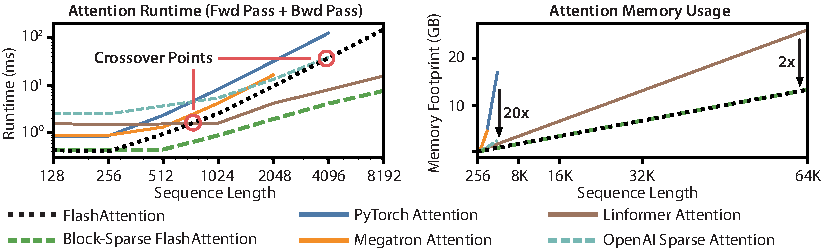
\includegraphics[width=5.5in]{figs/attention_benchmarks.pdf}
\iftoggle{arxiv}{}{
\vspace{-1em}
}
\caption{\textbf{Left:} runtime of forward pass + backward pass. \textbf{Right:} attention memory usage.}
\label{fig:benchmark}
\iftoggle{arxiv}{}{
\vspace{-1.0em}
}
\end{figure}



We vary sequence length and measure runtime and memory usage of \sysname and block-sparse \sysname against various attention baselines on one A100 GPU with 40 GB HBM, with dropout and a padding mask.
We compare against reference implementations for exact attention, approximate attention, and sparse attention.
We report a subset of baselines in the main body; Appendix~\ref{sec:experiment_details} contains more baselines and full details.




\paragraph{Runtime.}
Figure~\ref{fig:benchmark} (left) reports the runtime in milliseconds of the forward + backward pass of \sysname and block-sparse \sysname compared to the baselines in exact, approximate, and sparse attention (exact numbers in Appendix~\ref{sec:experiment_details}).
Runtime grows quadratically with sequence length, but \sysname runs significantly faster than \textbf{exact attention} baselines, up to 3$\times$ faster than the PyTorch implementation.
The runtimes of many approximate/sparse attention mechanisms grow linearly with sequence length, but \sysname still runs faster than approximate and sparse attention for short sequences due to fewer memory accesses.
The \textbf{approximate attention} runtimes begin to cross over with \sysname at sequences between 512 and 1024.
On the other hand, block-sparse \sysname is faster than all implementations of exact, sparse, and approximate attention that we know of, across all sequence lengths.

\paragraph{Memory Footprint.}
Figure~\ref{fig:benchmark} (right) shows the memory footprint of \sysname and block-sparse \sysname compared to various exact, approximate, and sparse attention baselines.
\sysname and block-sparse \sysname have the same memory footprint, which grows linearly with sequence length.
\sysname is up to 20$\times$ more memory efficient than \textbf{exact attention} baselines, and is more memory-efficient than the \textbf{approximate attention} baselines.
All other algorithms except for Linformer run out of memory on an A100 GPU before 64K, and \sysname is still 2$\times$ more efficient than Linformer.































